\chapter{Background research}

\section{AI image colourisation}

The problem of automated image colourisation from the previous century did not receive much attention. The process was carried out manually, mostly by artists. Back then, early photography lacked the developing agent which as a consequence made it more prone to quality deterioration due to the conditions of the environment. These environmental factors can be the humidity from the air, dust particles, temperature and mould. Other factors can be due to inappropriate storage, mishandling of images or improper image restoration process \cite{ware1994mechanism}. Additionally, early photography was in black and white, and the need for colourising them was in demand. Image restoration artists were often required to maintain these images and also enhance them (e.g add colourisation). 

It wasn't until this century when in 2004 when Anat Levin and Dani Lischinski proposed an automated solution \cite{Levin2004} that required users to scribble colours on a grayscale image, and then the process will apply the colour to regions across the image. 

\begin{figure}[H]
    \centering
    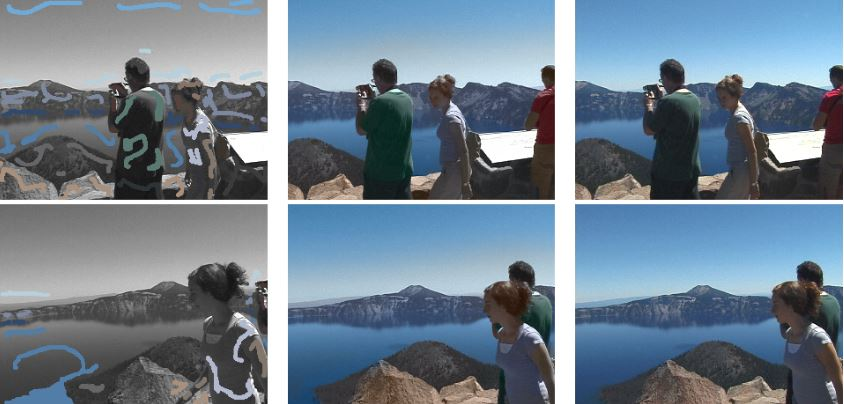
\includegraphics[width=0.6\columnwidth]{sections/figures/scribble_technique_colourisation.JPG}
    \caption{Anat Levin and Dani Lischinski's image colourisation method}
    \label{fig:my_label}
\end{figure}

This in turn significantly reduces the need for human intervention in the process of image colourisation. However, the limitation of Anat Levin and Dani Lischinski's method was that it was considered slow in producing the results. Over time, later research provided more automated methods for image colourisation. Whilst the methods provided by Anat Levin and Dani Lischinksi required one or several referenced images (provided by users or received automatically) as source data. The model learns to transfer colour across regions as shown in figure 2.1. 

On the other hand, newer methods involve a function that learns predictions from colour images from an extensive dataset during training, and the colourisation problem will either be a regression within the continuous colour space or a classification of colours with associated objects in the image. 




\subsection{Image colourisation projects}
This section goes over several existing projects relating to image colourisation.
\subsubsection*{Deoldify}
\addcontentsline{toc}{subsubsection}{Deoldify}
\textbf{Deoldify} is a well known black and white image colourisation library developed by Jason Antic\cite{jantic}. This project uses state of the art techniques such as GANS and has impressive colourisation results. Recently, Deoldify has developed a new type of GAN training method called No-GAN which is a model that addresses the many issues faced by his previous GAN model. A few of these issues are disruptive visual artefacts, bugs and inaccurate colouring. According to Jason Antic, the use of No-Gan has reportedly shown impressive results and achieves realistic colourisation.
\begin{figure}[H]
    \centering
    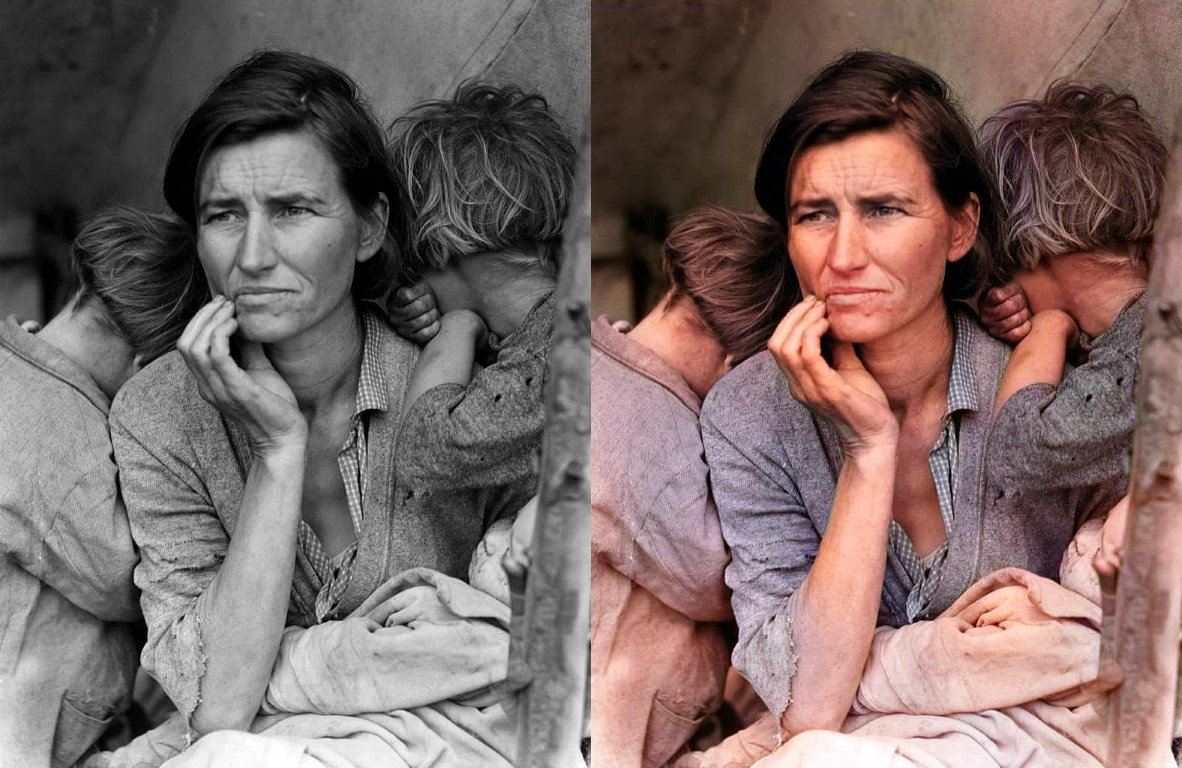
\includegraphics[width=0.7\columnwidth]{sections/figures/deoldify.jpg}
    \caption{Image colourised using Deoldify}
    \label{fig:my_label}
\end{figure}


\subsubsection*{Scribbler}
\addcontentsline{toc}{subsubsection}{Scribbler}
Scribbler (not to be confused with  Anat \& Dani's scribble method) is an interesting technique that involves turning pictures of sketches into realistic images using generative techniques\cite{sangkloy2016scribbler}. Even though their aim doesn't directly align with mine (image colourisation), their model can still generate realistic images with colours. They used a technique similar to \cite{Levin2004}, which involves user guidance by scribbling colours onto a sketch and will systematically apply those colours, whilst at the same time transforming the sketch into a realistic image. Their method is trained using in a GAN manner.
\begin{figure}[H]
    \centering
    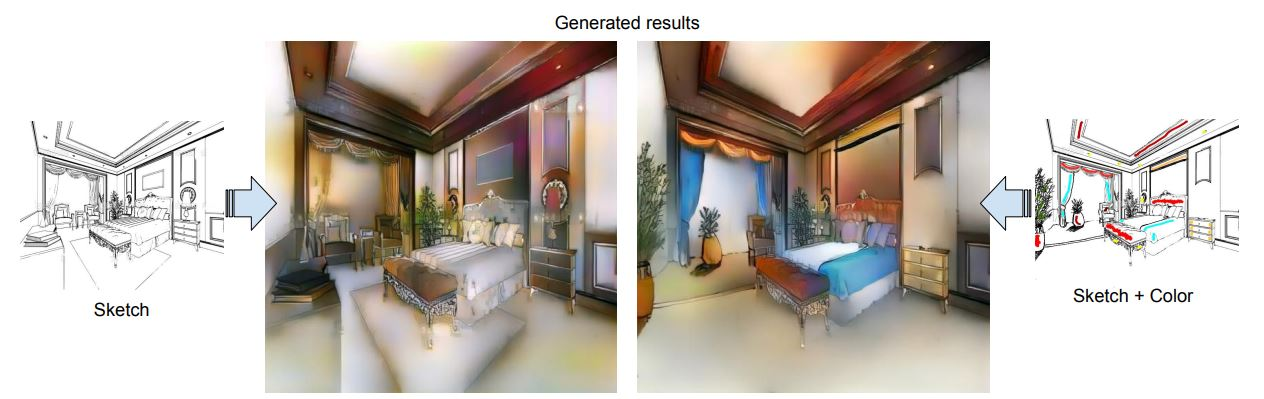
\includegraphics[width=0.7\columnwidth]{sections/figures/scribbler.JPG}
    \caption{Turning sketches into realistic images using Scribbler}
    \label{fig:my_label}
\end{figure}


\subsubsection*{Let there be Color!}
\addcontentsline{toc}{subsubsection}{Let there be Color!}
Similarly, "Let there be Color!" is another project that uses deep learning techniques to colourise black and white images, and is developed by \cite{IizukaSIGGRAPH2016}. They use an AutoEncoder which has been slightly modified to include a global feature extractor model. The addition of this modification meant the colourisation could be more accurate by applying relevant colours of the predicted class of the image. Their model has shown impressive colourisation results, as seen below in figure 2.3:
\begin{figure}[H]
    \centering
    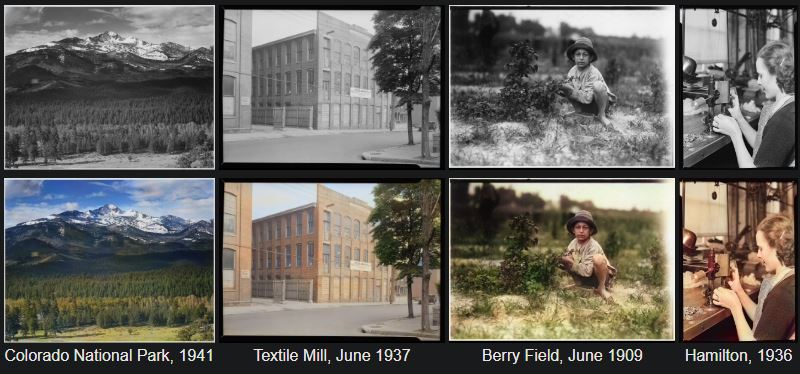
\includegraphics[width=0.7\columnwidth]{sections/figures/LTBC.JPG}
    \caption{Image colourisation results}
    \label{fig:my_label}
\end{figure}

\subsubsection*{End-to-End Image Colourisation}
\addcontentsline{toc}{subsubsection}{Pix2Pix}

The End-to-End conditional GAN-based image colourisation paper by \cite{inproceedings}. They use a conditional GAN architecture which is based on a well known cGAN architecture "Pix2Pix".

\begin{figure}[H]
    \centering
    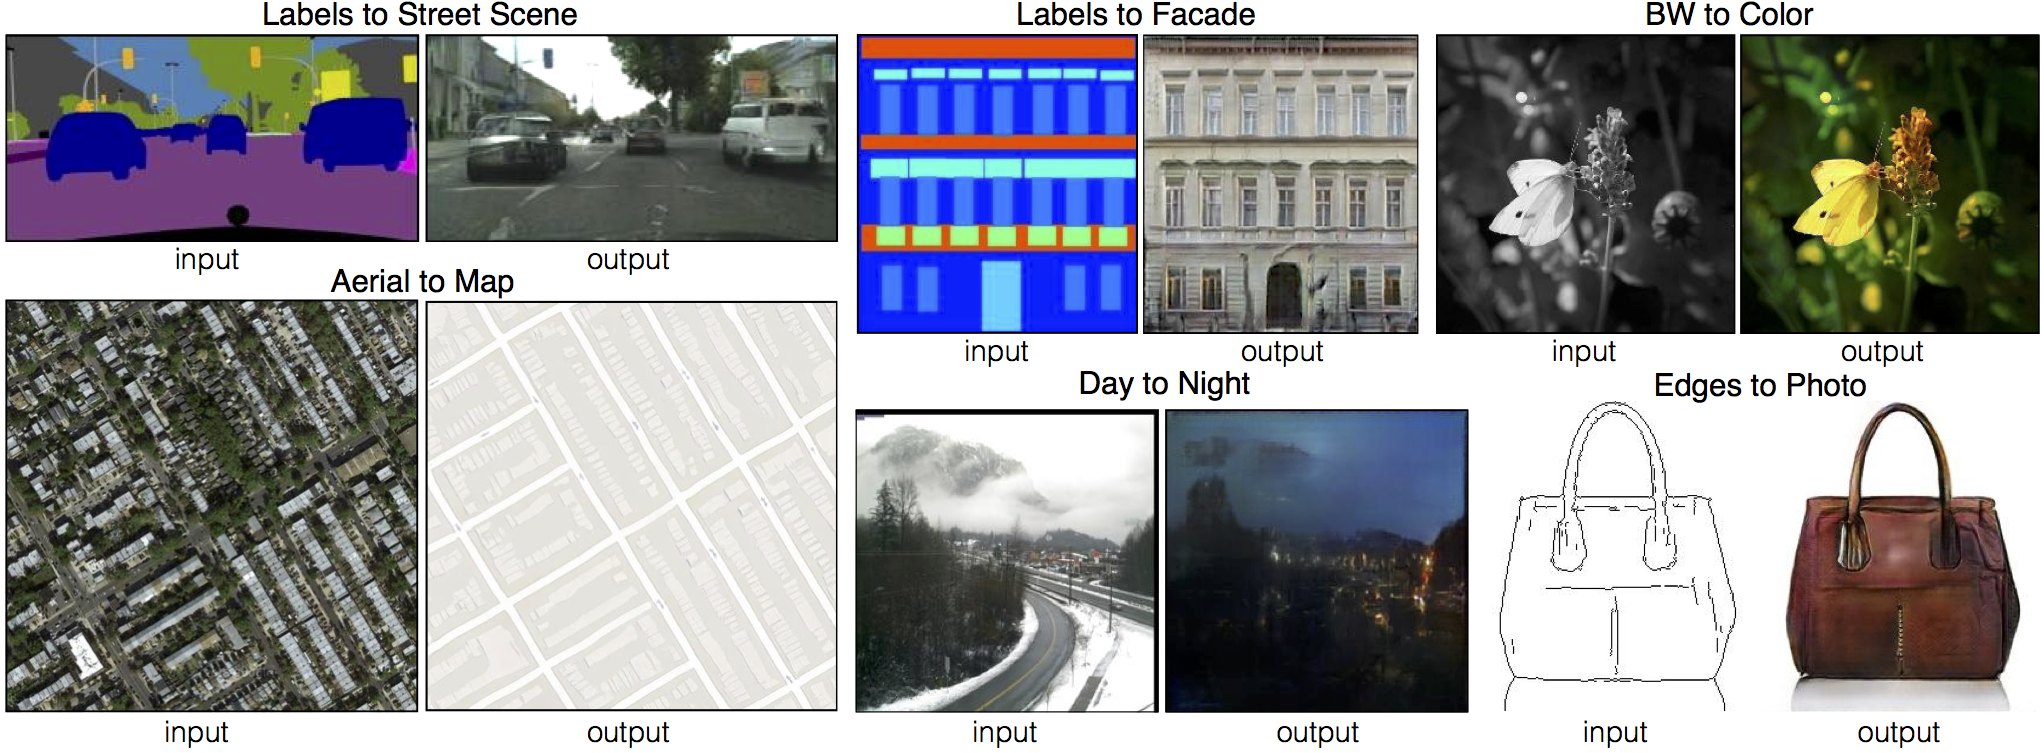
\includegraphics[width=0.7\columnwidth]{sections/figures/pix2pix.png}
    \caption{Pix2Pix image translation examples}
    \label{fig:my_label}
\end{figure}

Pix2Pix is a type of generative adversarial network used for image-to-image translation. Pix2Pix was presented by Phillip Isola in his 2016 paper \cite{DBLP:journals/corr/IsolaZZE16}. This architecture is used for many purposes that involve image-to-image translation as shown in the figure above. The author of End-to-End Image Colourisation decided to use this base architecture for image colourisation.




% For example, figure 2.5 shows the many possibilities Pix2Pix can achieve. For instance, it can be used to translate a sketch into a realistic photograph, Figure 2.5 also shows that a satellite image can be translated into something similar to google maps. Of course, the figure also demonstrates that image colourisation can be performed by translating black and white to its colour representation. The possibilities are quite endless as this architecture can be used to map nearly any arbitrary input to any arbitrary output.  

\subsubsection*{ChromaGAN}
\addcontentsline{toc}{subsubsection}{ChromaGAN}
The ChromaGAN is a conditional generative adversarial network proposed by the students from the University of Pompeu, Spain 2020 \cite{DBLP:journals/corr/abs-1907-09837}. Their proposal is primarily used for colourising grayscale images from semantic details engraved within the scene. Their method is an adaptation of \textbf{Let there be Color} since the generator of the architecture is inspired in the sense that it utilises a global feature extractor, but they decided to train this model in a GAN setting alongside a discriminator.

\begin{figure}[H]
    \centering
    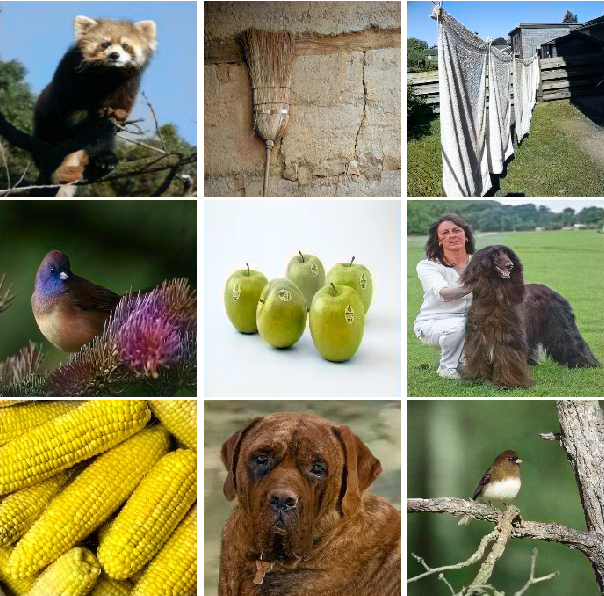
\includegraphics[width=0.5\columnwidth]{sections/figures/ChromaGAN.png}
    \caption{examples of ChromaGAN image colourisation}
    \label{fig:my_label}
\end{figure}




\subsection{Comparative literature review}


\begin{figure}[H]
    \centering
    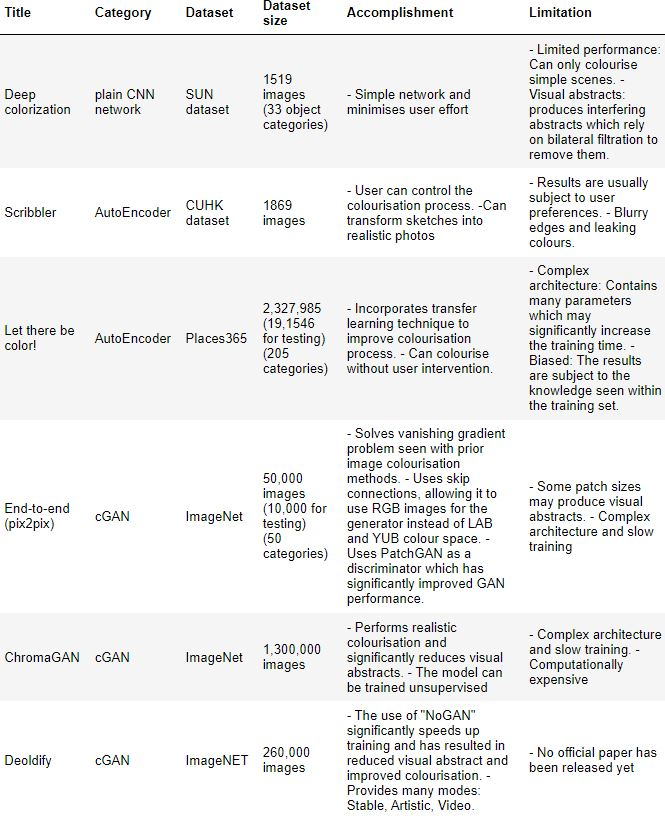
\includegraphics[scale=1,width=1\columnwidth]{sections/appendix/comparison.JPG}
    \caption{Advantages and disadvantages of each author's method}
    \label{fig:my_label}
\end{figure}

\subsection{RGB and LAB mapping}
In the task of image colourisation, the aim is to predict the colour channel of the given grayscale images. However in order to predict, a mapping between the grayscale pixel and the corrosponding coloured pixels is needed to be found defined colour space. 

\begin{figure}[H]
    \centering
    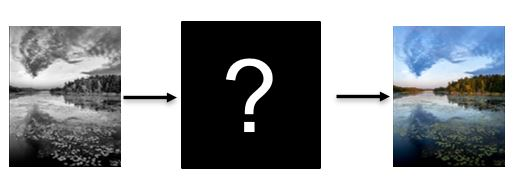
\includegraphics[width=0.7\columnwidth]{sections/figures/mapping.JPG}
    \caption{Image colourisation is a task of finding a mapping}
    \label{fig:my_label}
\end{figure}
As seen in the above figure, the task mainly involves finding a mapping such that a grayscale image (input) can be mapped to its corresponding coloured output. This mapping can be achieved by using a training set to discover all the related patterns used for mapping between grayscale and coloured. Here, the mapping can be achieved using two existing colour space representations: RGB and LAB.

% There exists a grey to colour mapping function \(F\) that can map the features contained at each pixel in a grayscale image \(L\) to learn the corresponding chrominance \(A*B*\) values from the image. The aim is to learn such a mapping function from the training set so that the conversion from grey to colour can be achieved using the function \(F\). 

\begin{figure}[H]
    \centering
    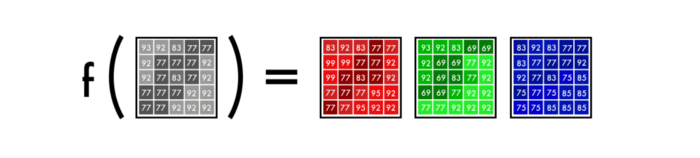
\includegraphics[width=0.6\columnwidth]{sections/figures/rgb.png}
    \caption{examples of ChromaGAN image colourisation \cite{wallner_2021}}
    \label{fig:my_label}
\end{figure}
One of the common representations is the RGB. This representation is widely used in electronic displays, such as computers, televisions, and cell phones. The RGB color model is an additive model in which red, green, and blue light are added together in different combinations to create a wide range of colors \cite{enwiki:1080368112}. For the task of colourisation, this representation will involve finding a mapping function to the three channels (as seen in the figure above). 


% \lipsum[1]
\begin{figure}[H]
    \centering
    
\includegraphics[width=0.6\columnwidth]{sections/figures/lab.png}
    \caption{examples of ChromaGAN image colourisation}
    \label{fig:my_label}
\end{figure}

There are other kinds of representations like LAB where L stands for luminance, and A and B for the colour spectra green–red and blue-yellow \cite{enwiki:1077444859}. Using the LAB colour channel in terms of image colourisation offers convenience as the L* channel represents the grayscale of the image and can be used as a conditional input. So while using the LAB representation, only 2 channels need to be mapped.


\pagebreak
\section{Similar Work}
\subsection{Human VS Objective evaluation of colorisation
performance}
Sean Mullery and Paul F. Whelan wrote a research investigation into evaluating image colourisation results using human and objective measures. Their research concerns more on whether the objective measures correlate with human opinion on images colourised using deep learning. They conducted a human evaluation test using Amazon mechanical Turk using 19 participants, and using their responses, they compared that against a dozen objective measures, to see if any of the objectives have a strong correlation with human opinion. 
The investigation concluded that the objective measures utilised in the colourisation literature did not correlate well with human opinion, with MS-SSIM showing the highest correlation, however, the correlation was too low to be considered an appropriate solution. They also reported on the behaviour of the observers, and noticed how most observers were tolerant to minor changes, but penalised heavily on medium to large changes \cite{https://doi.org/10.48550/arxiv.2204.05200}. 

\subsection{Image Colorization: A Survey and Dataset}
A comprehensive survey of various image colourisation methods was investigated by Saeed Anwar and Muhammad Tahir. This investigation was to address the need for a survey in the field of image colourisation. The survey involves the results of experiments on existing image colourisation methods. Here, they performed an extensive evaluation on several classes of architectures which are: Plain networks, user-guided networks, domain-specific networks, text-based networks, diverse colourisation networks, multi-path networks, and exemplar-based methods. Their investigation also discusses the many benefits and limitations of each existing colourisation method as well as mentions the same for datasets. Their report concluded that the current use of metrics used by many existing colourisation methods is inadequate to evaluate the colourisation, and also discovered how most image colourisation methods performed, such as how GAN-based methods delivered diverse colourisation whereas CNN-based methods tend to deliver sub-optimal results for complex scenes \cite{anwar2020ColorSurvey}. 

\subsection{A review of image colourisation}
A review of image colourisation was a report carried out by Bo Li, Yu-Kun Lai and Paul Rosin. Their paper discusses the history of image colourisation and goes on to mention automated-based image colourisation methods, with which they experimented. They perform an extensive evaluation of reference-based, user guidance-based and deep learning-based image colourisation methods and compare each method to see look for similarities and differences. Their report concluded that deep learning methods produced robust and meaningful results, however, were difficult to control. They also reported how no quantitative metrics exist to measure the quality of colourised results, mainly because how current metrics do not provide accurate measures for coloured images. They plan to investigate and develop a metric useful for coloured images as future work\cite{Li2019}.
\pagebreak
\section{Generative Neural Networks}
In deep learning there are neural networks and then there are generative neural networks. Here, I will only be mentioning the latter, so refer to Appendix B for information regarding Neural Networks.


\subsection{Auto encoder}
The autoencoder is a class of CNN, it is used to learn efficient coding of unlabeled data (unsupervised learning). Autoencoders attempt to learn representations (encoding) for a given set of data by decomposing the data into small bits of data (bottleneck). Then, the Autoencoder will use that representation to reconstruct (decoder) the original data \cite{IntroductionToAutoencoders}.
\begin{figure}[H]
    \centering
    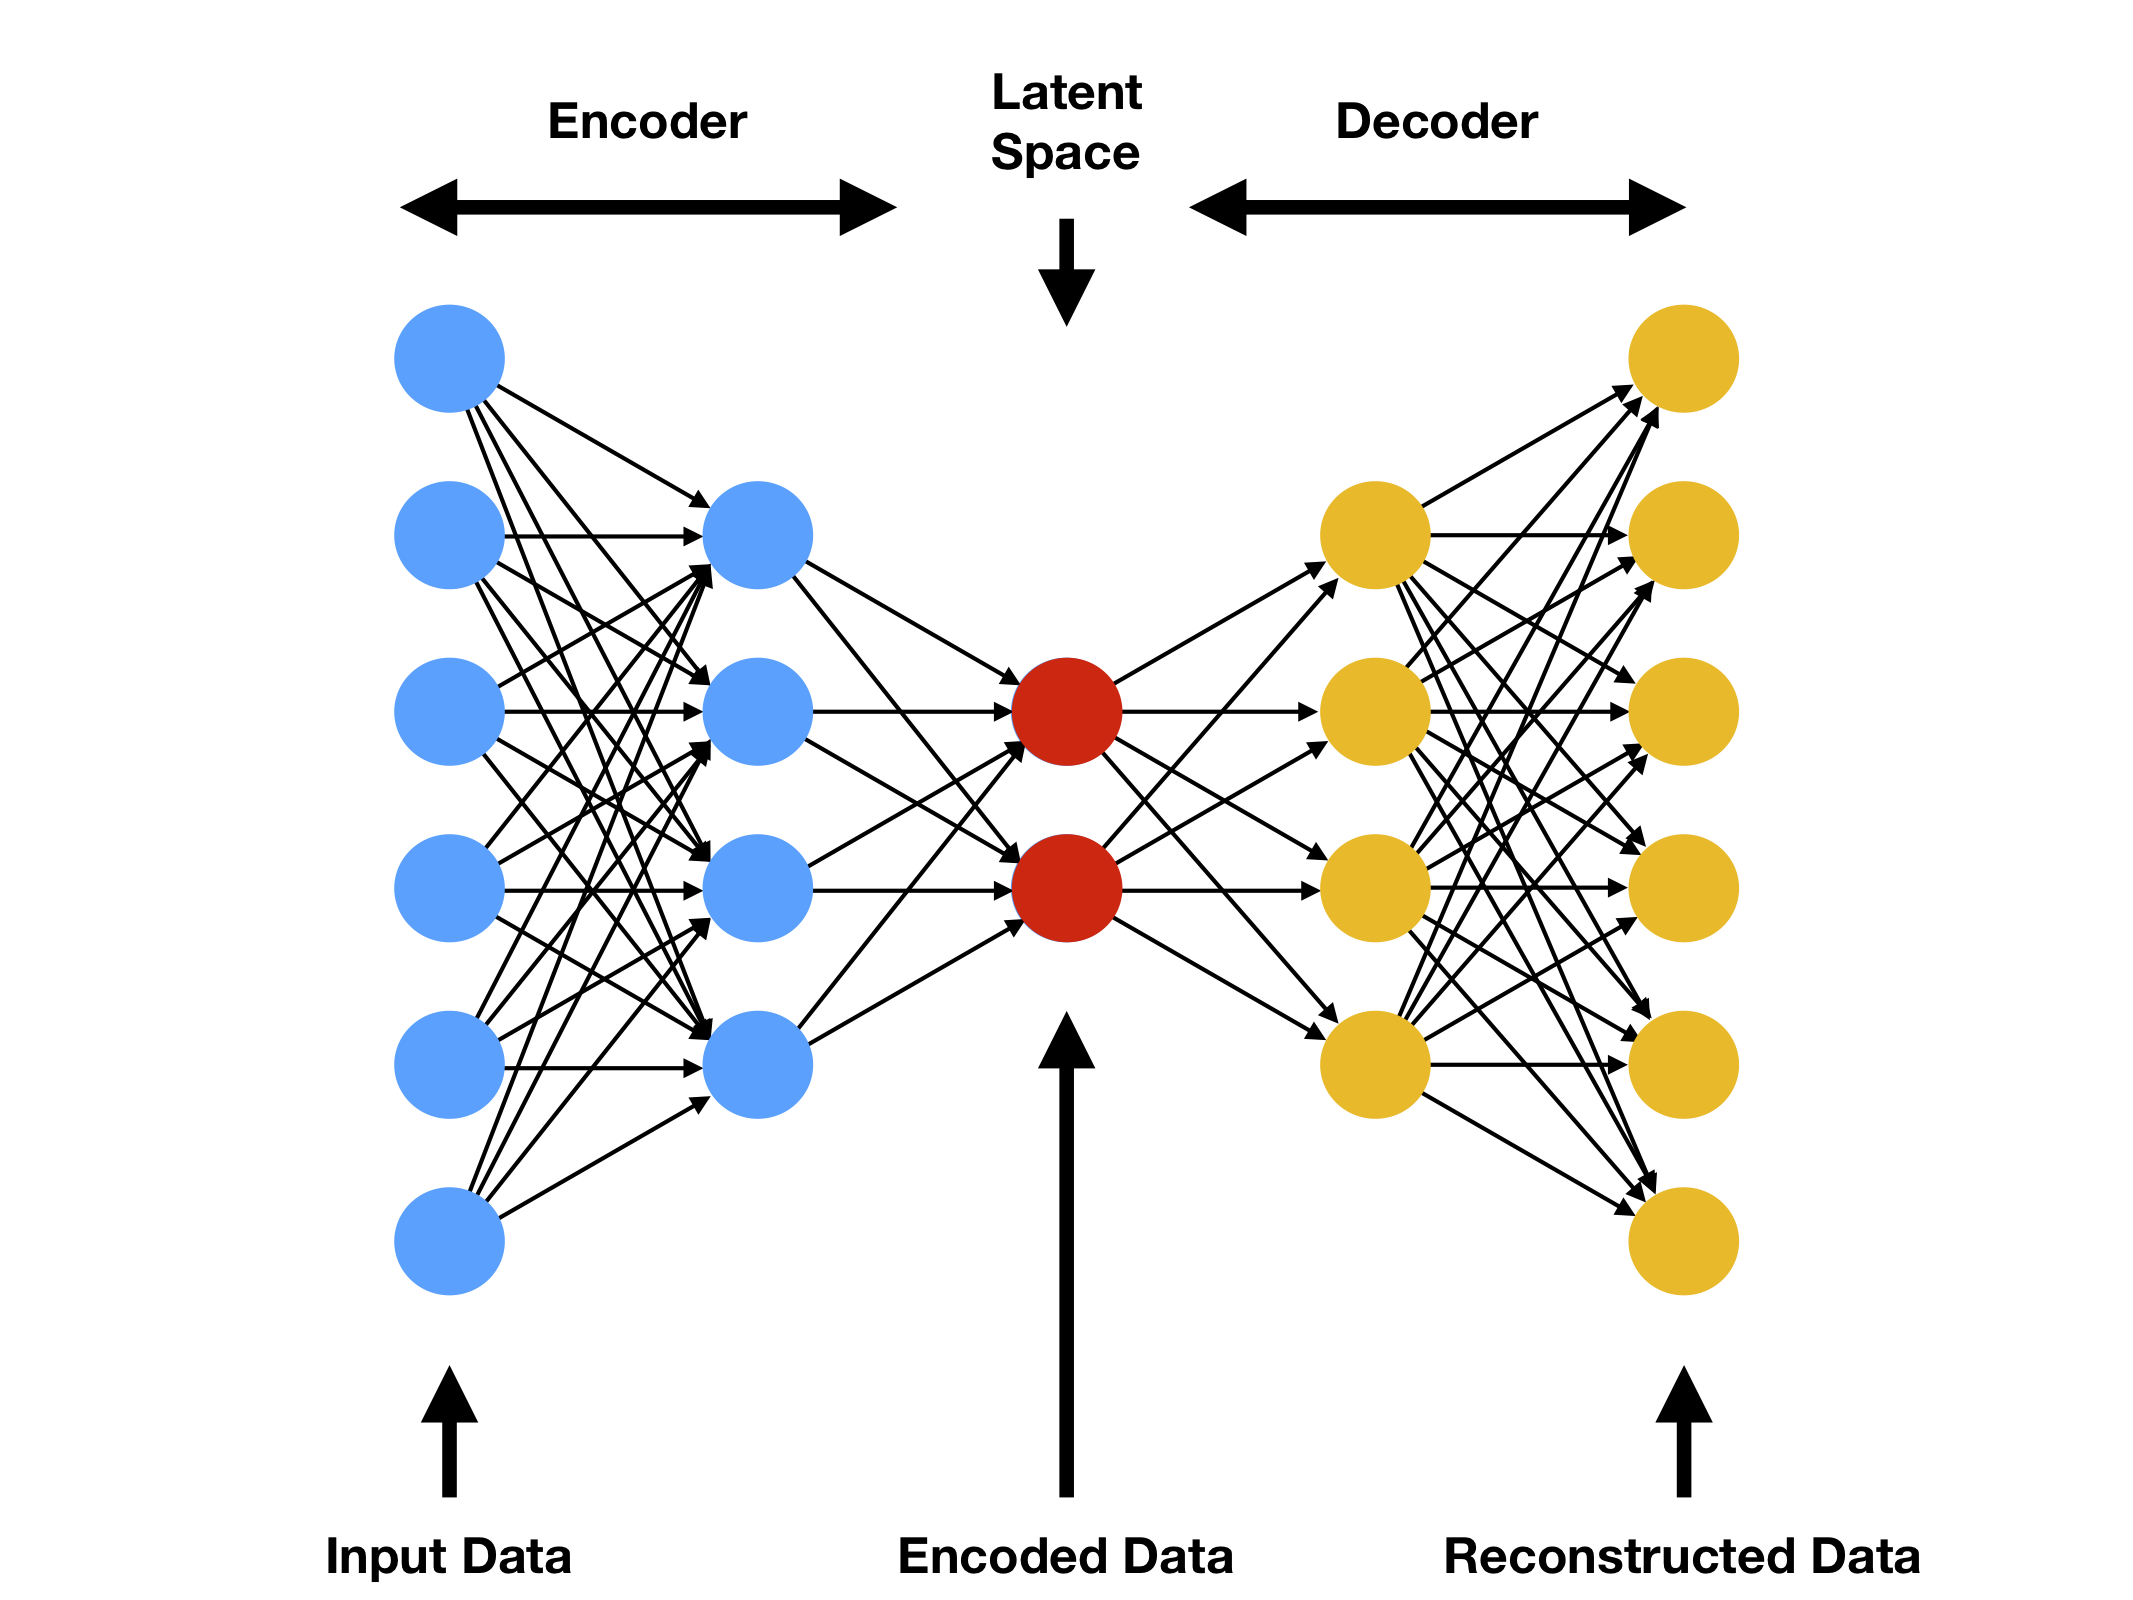
\includegraphics[width=0.6\columnwidth]{sections/figures/autoencoder_image.png}
    \caption{Example of an AutoEncoder model \cite{flores_2019}}
    \label{fig:my_label}
\end{figure}

\subsection{Generative Adversarial Networks}
A generative adversarial network (GAN) was introduced in 2014 by Goodfellow et al\cite{goodfellow2014generative}. The process of GAN involves a generator that generates an image, and its job is to fool the discriminator into thinking the generated image is real. As mentioned, the discriminator is used to determine whether the images presented by the generator are real or fake. If the image is deemed to be fake, the discriminator will pass feedback to the generator to suggest what the generator must do to improve its skill of making images that are indistinguishable from the real ones\cite{introToGanJasonBrownlee}. Both the generator and the discriminator are trained to outperform one another, eventually resulting in images that are increasingly realistic, making it impossible for the discriminator to tell the generated and the real images apart\cite{franoischollet2017learning}.
\begin{figure}[H]
    \centering
    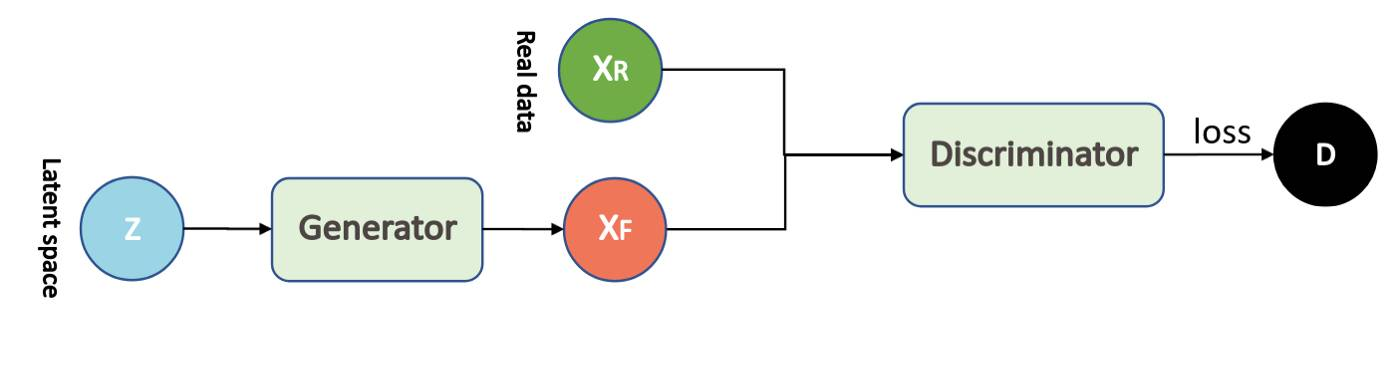
\includegraphics[width=0.7\columnwidth]{sections/figures/gan.JPG}
    \caption{Example of a gan model \cite{bagheri_2019}}
    \label{fig:my_label}
\end{figure}


\subsection{conditional GAN}
A cGan or conditional GAN is a generative adversarial network (GAN) that is conditioned on an additional input, typically an image. The cGan is different from a regular GAN in that it can generate images that are conditioned on a specific input, giving it the ability to generate images that are more realistic and diverse. The first cGan was developed by Mirza and Osindero in 2014. Some use cases for a cGan include generating realistic images, synthesizing images from text, and creating photo-realistic images\cite{frumkin_manipula_kachai_fehr_sewell}.
\begin{figure}[H]
    \centering
    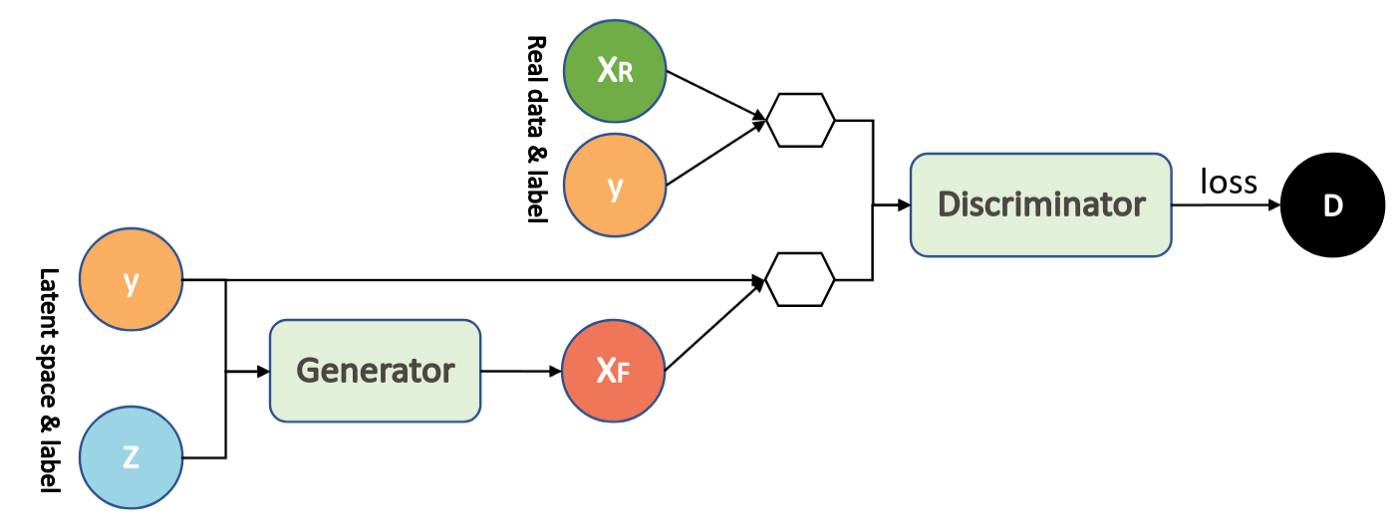
\includegraphics[width=0.7\columnwidth]{sections/figures/cgan.jpg}
    \caption{Example of a cGan model \cite{bagheri_2019}}
    \label{fig:my_label}
\end{figure}



\newpage
\section{Dataset}
In order for Machine learning models to understand how to perform various tasks, they'll first need to be trained using a sufficient amount of dataset. These datasets can be in various forms, such as numerical, categorical or time series, in my case I will be using numerical as it is a way of representing images. Datasets are often split up into 3 partitions: Training set which will be used to train the model; Validation set will be used to evaluate the model's performance during training; Testing set will be used to test the model's accuracy and performance after it has been trained. Since the models will perform image colourisation tasks, it'll need to be trained using an image dataset. Below are a few image datasets I have looked into that I can use to train the models:
\subsection{SUN dataset}
The Scene UNderstanding (SUN) dataset is a well-sampled dataset that contains about 130,519 annotated images spread over 899 categories \cite{sun}. The dataset is used by researchers specialising in the fields of computer vision, human perception, cognition, machine learning, and data science. Typically, the images in the dataset contain environmental scenes and everyday objects, which are all annotated with their corresponding category and name. The number of images in the SUN dataset is expanding constantly as new images are being annotated every day. In my case, this dataset provides a rich amount of images, which is already beyond the perfect amount needed to train the models.

\subsection{Places dataset}
The places dataset is an open-source large-scale image dataset used mainly for scene recognition in computer vision. The dataset contains 10 million scene photographs with annotations which makes it the largest existing scene-centric image dataset. This dataset is used in many applications within the world of computer vision, such as classification problems. The dataset contains a large number of natural images from a variety of places, including indoor and outdoor scenes. The dataset is divided into 365 categories, and each category contains a large number of images.\cite{Zhou1109}.


\subsection{Open Images Dataset}
The open images dataset is an open-source image dataset from Google. This dataset contains a significant amount of over 9 million images with annotations. It contains a total of 16 million boxes for 600 object classes on 1.9 million images, which makes it the largest existing dataset with object location annotation \cite{2020}. Like the SUN dataset, the open image dataset is expanding every single day, with each release adding millions of more annotated images. 
\newpage

\section{Requirements}
\subsection{Tensorflow}
\textbf{Tensorflow} is a powerful library used for \textbf{numerical tensor computation} and is primarily used for \textbf{creating and deploying large-scale Machine Learning models} and offers a plethora of tools. The library was first released for open source in 2015 by Google Brain Team and is now regarded as one of the\textbf{ most popular deep learning frameworks} to this day\cite{10.5555/3153997}. 


\subsection{Keras}
\textbf{Keras} is an open-source, deep-learning python library \textbf{developed by François Chollet in 2015} \cite{franoischollet2017learning}. The framework provides an interface used for defining and training any kind of deep learning model. However, for tensor computation, Keras has to rely on a \textbf{backend engine} such as TensorFlow which makes Keras a \textbf{high-level framework}. 


\subsection{Scikit-learn}
\textbf{Scikit-learn} is an open-source machine learning library used for the Python programming language and was \textbf{released in 2007 by French Data Scientist David Cournapeau}. The library \textbf{features several machine learning algorithms for classification, regression and clustering}. Additionally, the library offers utilities for applying transformations to data such as \textbf{Lab2RGB} and \textbf{RGB2LAB} (which will be used for this throughout my research project). NumPy is utilised for performing high-performance linear algebra and array operations \cite{enwiki:1065626908}.

\subsection{OpenCV}
\textbf{OpenCV} is an open-source multi-platform \textbf{computer vision library} that you can use to implement \textbf{object recognition, object tracking, 3D reconstruction, image matching, and image stitching}. It provides many powerful image processing and computer vision functions. It is \textbf{widely used by developers to develop computer vision} and machine learning applications\cite{enwiki:1072564905}.






